d) Suponga que $com(n,k)$ representa la cantidad de
diferentes comités de k personas que pueden formarse,
dadas n personas entre las cuales elegir. Por ejemplo,
$com(4,3) = 4$, porque dadas cuatro personas $A$,$B$,
$C$ y $D$ hay cuatro comités de tres personas posibles:
$ABC$, $ABD$, $ACD$ y $BCD$. Se puede comprobar la identidad:
\newline\hspace*{5mm}
$com(n,k) = com(n-1,k) + com(n-1,k-1)$
\newline
Escribir y probar un programa recursivo para calcular
$com(n,k)$ para $n,k >= 1$.
\lstinputlisting{Recursion/TareaD.c}
Capturas de Pantalla de Recursion/TareaD.c
\newline
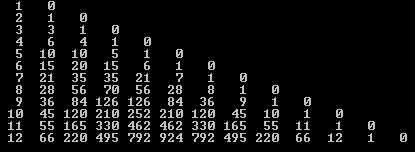
\includegraphics{Recursion/img/TareaD_1.png}